\documentclass[../main.tex]{subfiles}

\begin{document}

\section{Casual Inference}
  \begin{itemize}
    \item Inferring the effects of any treatment/policy/intervention/etc.
    \begin{itemize}
      \item effect of treatment on a disease
      \item effect of social media on health
    \end{itemize}
    \item Simpson's Paradox: mortality rate table
    \item Total population vs subgroup by conditions
    \item Correlation does not imply causation!
    \item Correlation: linear statistical dependence
    \item Association is the more correct term for statistical dependence
    \item It is possible to have large amounts of association with only \textit{some} being casual. Some association and 0 causation is a case of "assocation is not casuation"
    \item e.g.Wearing shoes and waking up with a headache, common cause of drinking the night before
    \item This is a "confoundeer", this is a type of \textit{confounding association}
    \item If association is causation, then causual inference could be solved using traditional statistics and ML
    \item Even with infinite amounts of data, we sometimes cannot compute casual quantities
    \item Identification of casual effects
    \item Intervention vs. observation. If we can intervene/experiment, identification becomes easy. Observational data is challenging because there is often confounding.
  \end{itemize}
  \subsection{Potential Outcomes}
    \begin{itemize}
      \item The \textit{potential outcome} $Y(t)$ denotes what your outcome would be if you were to take treatment $t$
      \item Potential outcomes aren't always observed, they can be potentially observed
      \item The one that is actually observed depends on the treatment
      \item Individual treatment effect (ITE) for the ith individual
      \begin{equation*}
        \tau_{i} \triangleq Y_{i}(1) - Y_{i}(0)
      \end{equation*}
      \item Fundamental problem of causal inference: can't observe all potential outcomes for a given individual, we cannot observe both $Y(1)$ and $Y(0)$
      \item The outcomes that you can't observe are called \textit{counterfactuals}
      \item Average treatment effect (ATE)
      \begin{equation*}
        \tau \triangleq \mbb{E}[Y_{i}(1) - Y_{i}(0)] = \mbb{E}[Y(1) - Y(0)]
      \end{equation*}
      \item Association difference is not the same as causal difference due to confounding
      \begin{equation*}
        \mbb{E}[Y|T=1] - \mbb{E}[Y|Y=0] \neq \mbb{E}[Y(1)] - \mbb{E}[Y(0)]
      \end{equation*}
    \end{itemize}
  \subsection{Ignorability and Exchangability}
    \begin{itemize}
      \item Ignorability - ignoring missing data, remove causal arrow from confounder to treatment
      \item Ignorability allows us to reduce ATE to associational difference
      \item Exchangability - treatment groups are exchangable such that if they were swapped, the new treatment group would observe the same outcome as the old treatment group
      \item Identifying a casual effect is to reduce causal expression to a statistical expression
      \item Conditional exchangability means if we condition on the covariate $X$, there is no longer any non-causal association between $T$ and $X$.
      \begin{figure}[h]
        \caption{Causal graphical models}
        \centering
        \begin{subfigure}{.5\textwidth}
          \centering
          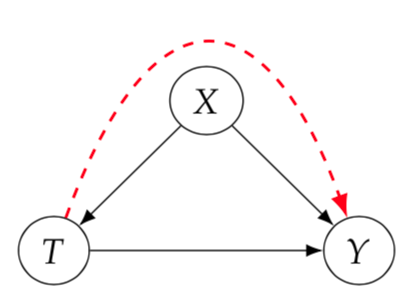
\includegraphics[width=.7\linewidth]{../imgs/confounding.png}
          \caption{$X$ is confounding the effect of $T$ on $Y$}
          \label{fig:confounding}
        \end{subfigure}%
        \begin{subfigure}{.5\textwidth}
          \centering
          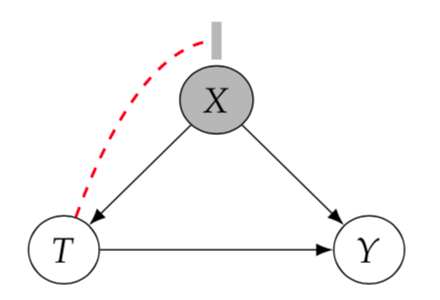
\includegraphics[width=.7\linewidth]{../imgs/blocking.png}
          \caption{Conditioning on $X$ leads to no confounding}
          \label{fig:blocking}
        \end{subfigure}
      \end{figure}
      \item Adjustment formula: Given the assumptions of unconfoundedness, positivity, consistency, and no interference, we can identify the ATE:
      \begin{equation*}
        \mbb{E}[Y(1) - Y(0)] = \mbb{E}_{X}[\mbb{E}[Y|T=1, X]- \mbb{E}[Y|T=0,X]]
      \end{equation*}
      \item Positivity-unconfoundedness tradeoff: conditioning on more covariates can lead to better chance of satisfying unconfoundedness, but it can lead to a higher chance of violating positivity
      \item No interference: $Y_{i}(t_{1},\cdot, t_{n} = Y_{i}(t_{i})$ otherwise my outcome is only a function of my own treatment
      \item Consistency: If treatment is T, then th observed outcome Y is the potential outcome under T. $T = t \rightarrow Y = Y(t)$
      \item Often we use a model (e.g. linear regression or some ML predictor) in place of conditional expectations $\mbb{E}[Y|T=t, X=x]$, these models are known as \textit{model-assisted estimators}.
    \end{itemize}
  \subsection{Definitions}
    \begin{itemize}
      \item Estimand: quantity that we want to estimate
      \item Estimate: is an approximation of some estimand
      \item Estimator: a function that maps a dataset to an estimate of an estimand
      \item Casual estimand: any estimand that contains a potential outcome
      \item Statistical estimand: any estimand that does not contain a potential outcome
      \begin{figure}[h]
        \caption{Identification Flowchart}
        \centering
        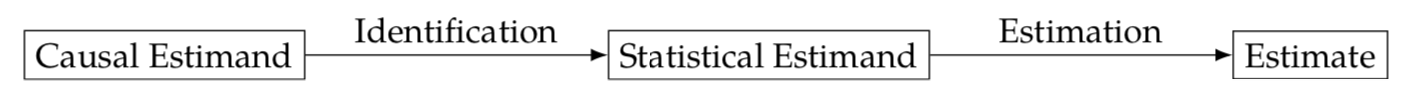
\includegraphics[width=1\textwidth]{../imgs/identification.png}
      \end{figure}

      \item Graph Terminology:
        \begin{itemize}
          \item A \textbf{graph} is a collection of \textbf{nodes} and \textbf{edges} that connect the nodes
          \item Undirected graphs: edges don't have any direction
          \item Directed graphs: edges go from a \textit{parent} node to a \textit{child} node, parents of node $X$ are pa($X$)
          \item Two nodes are \textit{adjacent} if they're connected by an edge
          \item A \textit{path} is any sequence of adjacent nodes regardless of direction, vs. a \textit{directed path}
          \item $X$ is an \textit{ancestor} of $Y$, and $Y$ is a \textit{descendant} of $X$
          \item Cycle
          \item If there are no cycles in a graph, then it is a \textit{directed acyclic graph} (DAG)
        \end{itemize}
      \item Bayesian Networks
        \begin{itemize}
          \item An intuitive way to model many variables together in a joint distribution is to only model local dependencies
          \item Local Markov Assumption: given its parents in the DAG, a node $X$ is independent of its non-descendants
          \item Bayesian Network Factorization: given a probability $P$ and a DAG $G$, $P$ factorizes according to $G$ if
          \begin{equation*}
            P(x_{1}, \cdot, x_{n}) = \prod_{i} P(x_{i}|pa_{i})
          \end{equation*}
          \item Also known as the \textit{chain rule for Bayesian networks}
        \end{itemize}
      \item Minimal Assumption: also adds that adjacant nodes in the DAG are dependent, also equivalent to saying that we can't remove any more edges from the graph
    \end{itemize}
  \subsection{Causal Graphs}
    \begin{itemize}
      \item A variable $X$ is said to be a cause of variable $Y$ if $Y$ can change in response to changes to $X$
      \item In a DAG, every parent is a direct cause of all of its children
      \begin{figure}[h]
        \caption{Graph building blocks}
        \centering
        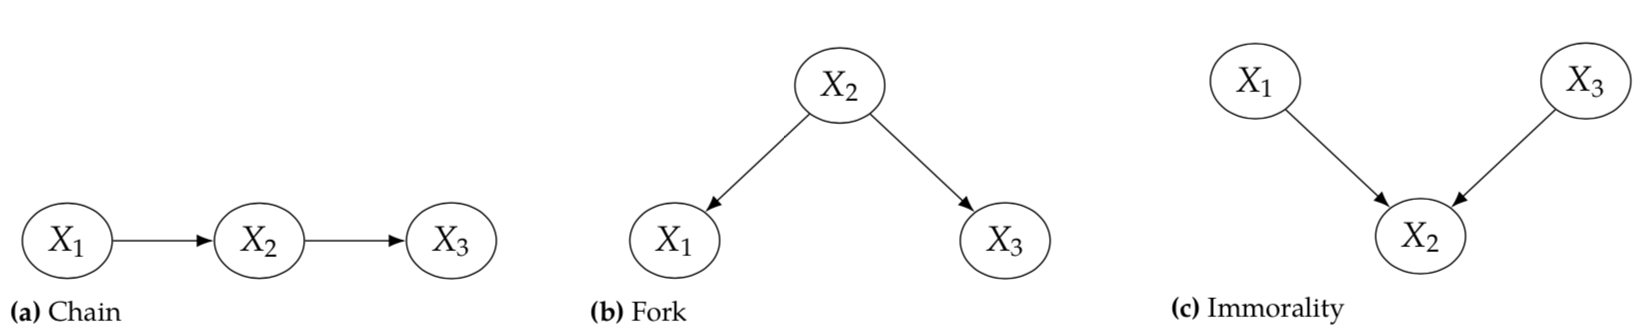
\includegraphics[width=1\textwidth]{../imgs/graph_blocks.png}
      \end{figure}
      \item Two unconnected nodes are conditionally independent. $P(x_{1}, x_{2}) = P(x_{1})P(x_{2})$
      \item $X_{1}$ and $X_{3}$ are associated in chains and forks because they're commonly associated with $X_{2}$
      \item When we condition on $X_{2}$ for forks and chains, it blocks the flow of association because of the local Markov Assumption
      \begin{figure}[h]
        \caption{Causal graphical models}
        \centering
        \begin{subfigure}{.33\textwidth}
          \centering
          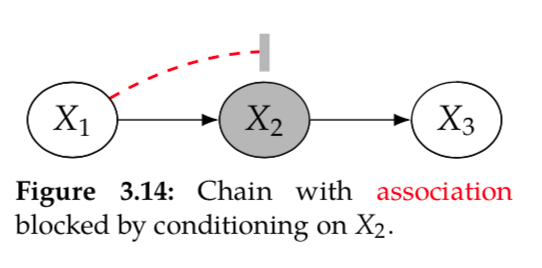
\includegraphics[width=0.8\linewidth]{../imgs/chain_block.png}
          \label{fig:chain_block}
        \end{subfigure}%
        \begin{subfigure}{.33\textwidth}
          \centering
          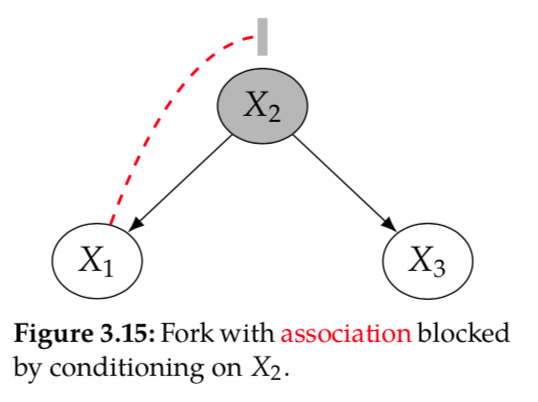
\includegraphics[width=0.8\linewidth]{../imgs/fork_block.png}
          \label{fig:fork_block}
        \end{subfigure}
        \begin{subfigure}{.33\textwidth}
          \centering
          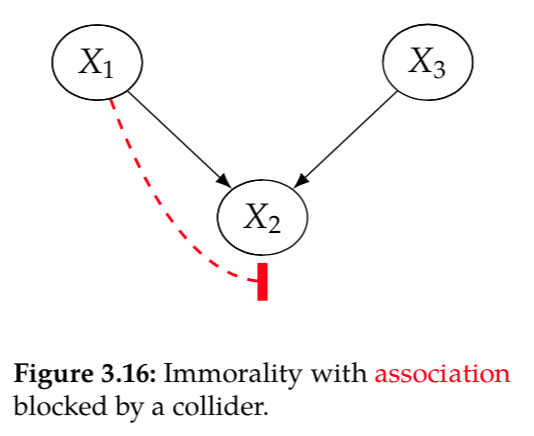
\includegraphics[width=0.8\linewidth]{../imgs/immorality.png}
          \label{fig:immorality}
        \end{subfigure}
      \end{figure}
      \item Colliders child of two parents that are not connected by an edge. In a collider, the parents are independent e.g. $X_{1} \ind X_{3}$, this is a \textit{blocked path}
      \item When we condition on a collider ($X_{2}$), its parents $X_{1}$ and $X_{3}$ become dependent
      \item Conditioning on a collider can turn a \textit{blocked path} to an \textit{unblocked path}
      \item This phenomenon is known as \textit{Berkson's paradox}
      \item Conditioning on descendants of a collider also induces association between parents of the collider
      \item In causal graphs, the edges have causal meaning
    \end{itemize}

  \subsection{d-separation}
    \begin{itemize}
      \item Two sets of nodes $X$ and $Y$ are d-separated by a set of nodes $Z$ if all of the paths between $X$ and $Y$ are blocked by $Z$
      \item If all paths between $X$ and $Y$ are blocked, then they are \textit{d-separated}
      \item D-separation implies conditional independence
      \item Global markov assumption: $X \ind_{G} Y | Z \implies X \ind_{P} Y | Z$
      \item Conditioning on $T = t$ means we restrict focus to subset of population to those who receive treatment $t$
      \item Intervention: take whole population and give everyone treatment $t$
      \item Denote intervention using $do(T = t)$ operator
      \item Interventional distribution: $P(Y|do(t))$ vs observational distribution: $P(Y)$
      \item
    \end{itemize}

  \subsection{Structural Causal Models (SCMs)}
    \begin{itemize}
      \item Structural equation: $B := f(A, U)$
      \item $:=$ gives us casual relation, A causes B
      \item $\mcal{U}$ is some unobserved random variable and denotes all the relevant (noisy) background conditions that cause B
      \begin{align*}
        B &:= f_{B}(A, \mcal{U}_{B}) \\
        C &:= f_{C}(A, B, \mcal{U}_{C}) \\
        D &:= f_{D}(A, C, \mcal{U}_{D}) \\
      \end{align*}
      \item The variables that we write structural equations for are \textit{endogenous} variables, these are the variables whose causal mechanisms we are modeling, $\{B, C, D\}$
      \item \textit{Exogenous} variables are variables who don't have any parents in the causal graph, $\{A, \mcal{U}_{\{B, C, D\}}\}$
      \item A structural casual model is a tuple of:
      \begin{itemize}
        \item A set of endogenous variables $V$
        \item A set of exogenous variables $U$
        \item A set of functions $f$ to generate each endogenous variable as a function of other variables
      \end{itemize}
      \item If casual graph has no cycles and noise variables are independent then it is \textit{Markovian}, if noise terms are dependent then it is \textit{semi-Markovian}
      \item Intervention $do(T=t)$, replace structural equation for $T$ with $T:=t$, then we get the \textit{interventional SCM $M_{t}$}
      \item This is by the modularity assumption

    \end{itemize}





\section{Bayesian Inference}

\section{Variational Inference}

\section{Expectation Maximization}
  \begin{itemize}
    \item Parameters $\theta$, evidence $X$
    \item Prior: probability of parameters, $p(\theta)$
    \item Likelihood: probability of evidence given parameters, $p(X | \theta)$
    \item Posterior: probability of the parametersgiven evidence, $p(\theta | X)$
    \begin{align*}
      p(\theta|x) &= \frac{p(x|\theta)}{p(x)}p(\theta) \\
      posterior &= \frac{likelihood}{constant}{prior}
    \end{align*}
    \item Maximum a posteriori estimate (MAP): estimate of an unknown quantity, mode of a posterior distribution
    \item point estimate of unobservable quantity based on empirical data

    \item EM: iterative method to find maximum likelihood or maximum a posteriori (MAP) estimate of parameters in a statistical model

    \item alternate between Expectation step and Maximization step
    \item E-step: creates a function for expectation of log-likelihood evaluated using current estimates of parameter
    \item M-step: computes new parameters that maximize expected log-likelihood
  \end{itemize}

\end{document}